\documentclass[border=3pt]{standalone}
% Shared TikZ styles for all paper figures.
%
% Colour is used to separate the two views (logical = blue, physical = ochre)
% and to mark the one emphasised relation (rose). Shape, line style and weight
% carry the same distinctions independently, so the figures still read when
% printed in black and white -- see the greyscale check in `make gray`.
\usepackage{tikz}
\usepackage{amsmath}
\usepackage[scaled=0.92]{helvet}
\renewcommand{\familydefault}{\sfdefault}
% Define \GRAYFIGS before % Shared TikZ styles for all paper figures.
%
% Colour is used to separate the two views (logical = blue, physical = ochre)
% and to mark the one emphasised relation (rose). Shape, line style and weight
% carry the same distinctions independently, so the figures still read when
% printed in black and white -- see the greyscale check in `make gray`.
\usepackage{tikz}
\usepackage{amsmath}
\usepackage[scaled=0.92]{helvet}
\renewcommand{\familydefault}{\sfdefault}
% Define \GRAYFIGS before % Shared TikZ styles for all paper figures.
%
% Colour is used to separate the two views (logical = blue, physical = ochre)
% and to mark the one emphasised relation (rose). Shape, line style and weight
% carry the same distinctions independently, so the figures still read when
% printed in black and white -- see the greyscale check in `make gray`.
\usepackage{tikz}
\usepackage{amsmath}
\usepackage[scaled=0.92]{helvet}
\renewcommand{\familydefault}{\sfdefault}
% Define \GRAYFIGS before \input{figstyle} to build the same figures in
% greyscale (xcolor converts every colour below), e.g.
%   pdflatex -jobname=fig1_gray "\def\GRAYFIGS{}\input{fig1_concept}"
\ifdefined\GRAYFIGS
  \usepackage[gray]{xcolor}
\else
  \usepackage{xcolor}
\fi
\usetikzlibrary{arrows.meta,positioning,fit,backgrounds,calc,shapes.geometric,
                shapes.misc,decorations.pathreplacing,patterns,matrix,shadows.blur}

% ------------------------------- palette -----------------------------------
\definecolor{ink}{HTML}{22333F}        % primary text
\definecolor{inkSoft}{HTML}{6B8299}    % secondary text, hairlines
\definecolor{astLine}{HTML}{2C7A9B}    % logical view
\definecolor{astFill}{HTML}{E7F2F7}
\definecolor{pdfLine}{HTML}{B0762F}    % physical view
\definecolor{pdfFill}{HTML}{FBF2E3}
\definecolor{hotLine}{HTML}{B03A55}    % the emphasised relation
\definecolor{hotFill}{HTML}{FBE9EC}
\definecolor{mutedLine}{HTML}{9FB3C8}  % furniture / unmatched
\definecolor{mutedFill}{HTML}{F1F5F8}

\tikzset{
  every node/.append style = {text=ink},
  >=Stealth,
  % --- logical structure (AST) -------------------------------------------
  astnode/.style   = {draw=astLine!70, fill=white, rounded corners=2.5pt,
                      line width=0.6pt, font=\scriptsize,
                      inner xsep=4pt, inner ysep=2.5pt, minimum height=4.6mm},
  astroot/.style   = {astnode, fill=astLine, draw=astLine, text=white},
  astsec/.style    = {astnode, fill=astFill},
  asttree/.style   = {draw=astLine!50, line width=0.6pt, rounded corners=2.5pt},
  % --- physical layout (page regions) ------------------------------------
  page/.style      = {draw=inkSoft!45, fill=white, line width=0.6pt,
                      rounded corners=2pt},
  lbox/.style      = {draw=pdfLine!55, fill=white, line width=0.6pt,
                      rounded corners=1.2pt},
  lboxhi/.style    = {draw=hotLine, fill=hotFill, line width=1.0pt,
                      rounded corners=1.2pt},
  furniture/.style = {draw=mutedLine, dash pattern=on 1.6pt off 1.4pt,
                      fill=mutedFill, line width=0.6pt, rounded corners=1.2pt},
  % --- relations ----------------------------------------------------------
  maplink/.style   = {draw=inkSoft, line width=0.6pt,
                      -{Stealth[length=1.7mm,width=1.3mm]}},
  maphot/.style    = {draw=hotLine, line width=1.1pt,
                      -{Stealth[length=2mm,width=1.6mm]}},
  flow/.style      = {draw=inkSoft, line width=0.7pt,
                      -{Stealth[length=2mm,width=1.6mm]}, rounded corners=2pt},
  % --- pipeline stages ----------------------------------------------------
  stage/.style     = {draw=inkSoft!55, fill=white, rounded corners=2.5pt,
                      font=\scriptsize, align=center, inner sep=3.5pt,
                      minimum height=7mm, text width=32mm},
  artefact/.style  = {draw=inkSoft!35, fill=mutedFill, rounded corners=2.5pt,
                      font=\scriptsize, align=center, inner sep=3.5pt,
                      minimum height=7mm, text width=32mm},
  % --- labels -------------------------------------------------------------
  grouplbl/.style  = {font=\scriptsize, text=inkSoft},
  caption/.style   = {font=\scriptsize, text=ink},
  tinylbl/.style   = {font=\tiny, text=inkSoft},
  softcard/.style  = {rounded corners=4pt, draw=none},
}

% Fake text lines inside a layout box.
% [colour] {x} {y top} {width} {line count}
\newcommand{\fakelines}[5][pdfLine!32]{%
  \foreach \fli in {1,...,#5}{%
    \draw[#1, line width=0.32pt] (#2,{#3-0.115*\fli}) -- ++({#4},0);}%
}
% Same, with a short final line (end of a paragraph)
\newcommand{\fakepara}[5][pdfLine!32]{%
  \foreach \fli in {1,...,#5}{%
    \draw[#1, line width=0.32pt] (#2,{#3-0.115*\fli}) -- ++({#4},0);}%
  \draw[#1, line width=0.32pt] (#2,{#3-0.115*(#5+1)}) -- ++({0.55*#4},0);%
}
 to build the same figures in
% greyscale (xcolor converts every colour below), e.g.
%   pdflatex -jobname=fig1_gray "\def\GRAYFIGS{}\documentclass[border=3pt]{standalone}
\input{figstyle}
\begin{document}
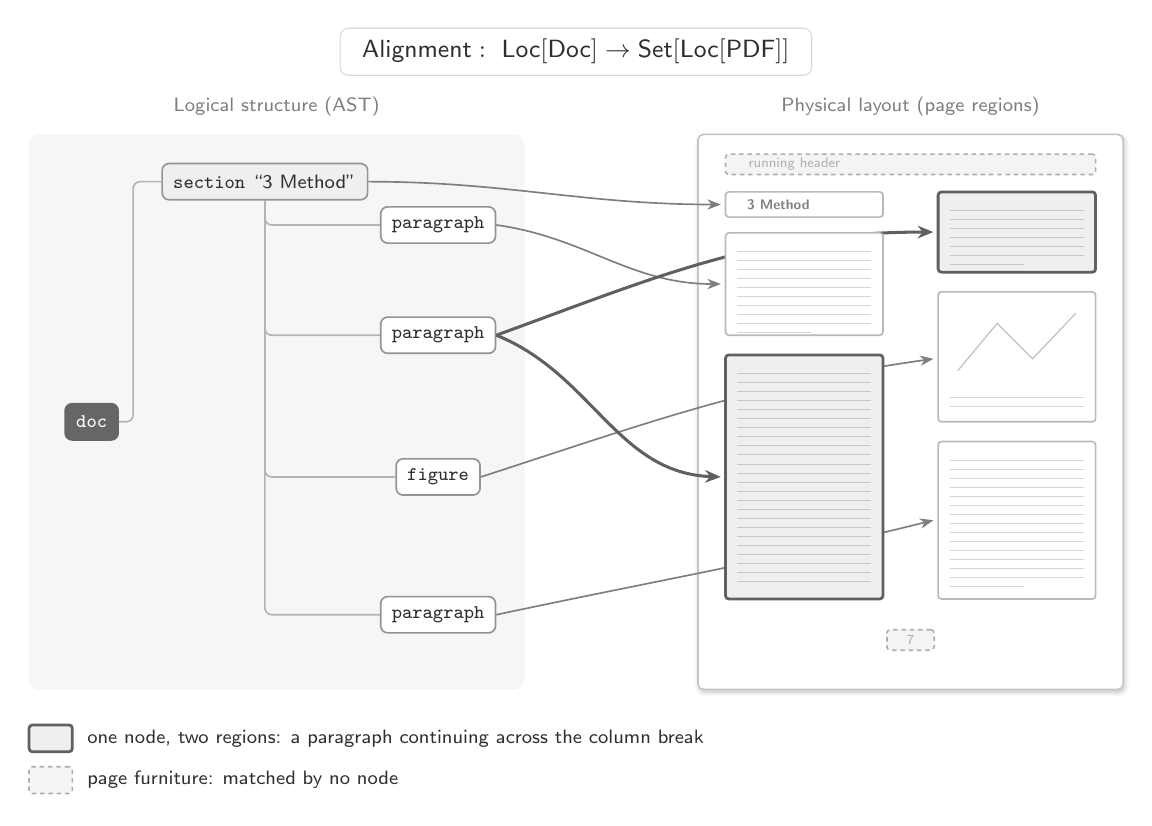
\begin{tikzpicture}

% ============================ title badge ==================================
\node[rounded corners=3pt, draw=inkSoft!30, fill=white, inner xsep=8pt,
      inner ysep=4pt, font=\small] at (6.95,8.00)
     {$\mathsf{Alignment}:\ \mathsf{Loc}[\mathsf{Doc}] \rightarrow
       \mathsf{Set}[\mathsf{Loc}[\mathsf{PDF}]]$};

\node[grouplbl] at (3.15,7.30) {Logical structure (AST)};
\node[grouplbl] at (11.20,7.30) {Physical layout (page regions)};

% ============================ the two cards ================================
\fill[softcard, fill=astFill!55] (0.00,-0.10) rectangle (6.30,6.95);
\node[page, fit={(8.50,-0.10) (13.90,6.95)}, inner sep=0pt,
      blur shadow={shadow blur steps=8, shadow xshift=0.5pt,
                   shadow yshift=-0.9pt, shadow opacity=25}] {};

% ======================= LEFT: logical structure (AST) =====================
\node[astroot] (doc)  at (0.80,3.30) {\texttt{doc}};
\node[astsec]  (sec1) at (3.00,6.35) {\texttt{section} ``3 Method''};
\node[astnode] (p1)   at (5.20,5.80) {\texttt{paragraph}};
\node[astnode] (p2)   at (5.20,4.40) {\texttt{paragraph}};
\node[astnode] (fg)   at (5.20,2.60) {\texttt{figure}};
\node[astnode] (p3)   at (5.20,0.85) {\texttt{paragraph}};

\draw[asttree] (doc.east) -- ++(0.18,0) |- (sec1.west);
\foreach \c in {p1,p2,fg,p3}{ \draw[asttree] (sec1.south) |- (\c.west); }

% ============================= THE MAPPING =================================
% (drawn before the regions, so the links pass behind them)
\draw[maplink] (sec1.east) to[out=0,in=180]   (8.79,6.06);
\draw[maplink] (p1.east)   to[out=-8,in=180]  (8.79,5.05);
\draw[maplink] (fg.east)   to[out=18,in=188]  (11.49,4.10);
\draw[maplink] (p3.east)   to[out=12,in=194]  (11.49,2.05);

% one node, two regions, split across the column break
\draw[maphot]  (p2.east) to[out=-22,in=178] (8.79,2.60);
\draw[maphot]  (p2.east) to[out=20,in=180]  (11.49,5.71);

% ======================= page regions (opaque, on top) =====================
\node[furniture, fit={(8.85,6.44) (13.55,6.70)}, inner sep=0pt] {};
\node[font=\tiny, text=mutedLine, anchor=west] at (9.02,6.57) {running header};
\node[furniture, fit={(10.90,0.40) (11.50,0.66)}, inner sep=0pt] {};
\node[font=\tiny, text=mutedLine] at (11.20,0.53) {7};

% --- left column ---
\node[lbox, fit={(8.85,5.90) (10.85,6.22)}, inner sep=0pt] {};
\node[font=\tiny, text=pdfLine, anchor=west] at (9.00,6.06) {\textbf{3 Method}};

\node[lbox, fit={(8.85,4.40) (10.85,5.70)}, inner sep=0pt] {};
\fakepara{9.00}{5.58}{1.70}{9}

\node[lboxhi, fit={(8.85,1.05) (10.85,4.15)}, inner sep=0pt] {};
\fakelines[hotLine!35]{9.00}{4.03}{1.70}{24}

% --- right column ---
\node[lboxhi, fit={(11.55,5.20) (13.55,6.22)}, inner sep=0pt] {};
\fakepara[hotLine!35]{11.70}{6.10}{1.70}{6}

\node[lbox, fit={(11.55,3.30) (13.55,4.95)}, inner sep=0pt] {};
\draw[pdfLine!45, line width=0.5pt, line join=round]
      (11.80,3.95) -- (12.30,4.55) -- (12.75,4.10) -- (13.30,4.68);
\fakelines{11.70}{3.72}{1.70}{2}

\node[lbox, fit={(11.55,1.05) (13.55,3.05)}, inner sep=0pt] {};
\fakepara{11.70}{2.93}{1.70}{14}

% ================================ legend ===================================
\node[lboxhi, minimum width=5.5mm, minimum height=3.4mm, inner sep=0pt]
      at (0.28,-0.72) {};
\node[caption, anchor=west] at (0.62,-0.72)
     {one node, two regions: a paragraph continuing across the column break};

\node[furniture, minimum width=5.5mm, minimum height=3.4mm, inner sep=0pt]
      at (0.28,-1.25) {};
\node[caption, anchor=west] at (0.62,-1.25)
     {page furniture: matched by no node};

\end{tikzpicture}
\end{document}
"
\ifdefined\GRAYFIGS
  \usepackage[gray]{xcolor}
\else
  \usepackage{xcolor}
\fi
\usetikzlibrary{arrows.meta,positioning,fit,backgrounds,calc,shapes.geometric,
                shapes.misc,decorations.pathreplacing,patterns,matrix,shadows.blur}

% ------------------------------- palette -----------------------------------
\definecolor{ink}{HTML}{22333F}        % primary text
\definecolor{inkSoft}{HTML}{6B8299}    % secondary text, hairlines
\definecolor{astLine}{HTML}{2C7A9B}    % logical view
\definecolor{astFill}{HTML}{E7F2F7}
\definecolor{pdfLine}{HTML}{B0762F}    % physical view
\definecolor{pdfFill}{HTML}{FBF2E3}
\definecolor{hotLine}{HTML}{B03A55}    % the emphasised relation
\definecolor{hotFill}{HTML}{FBE9EC}
\definecolor{mutedLine}{HTML}{9FB3C8}  % furniture / unmatched
\definecolor{mutedFill}{HTML}{F1F5F8}

\tikzset{
  every node/.append style = {text=ink},
  >=Stealth,
  % --- logical structure (AST) -------------------------------------------
  astnode/.style   = {draw=astLine!70, fill=white, rounded corners=2.5pt,
                      line width=0.6pt, font=\scriptsize,
                      inner xsep=4pt, inner ysep=2.5pt, minimum height=4.6mm},
  astroot/.style   = {astnode, fill=astLine, draw=astLine, text=white},
  astsec/.style    = {astnode, fill=astFill},
  asttree/.style   = {draw=astLine!50, line width=0.6pt, rounded corners=2.5pt},
  % --- physical layout (page regions) ------------------------------------
  page/.style      = {draw=inkSoft!45, fill=white, line width=0.6pt,
                      rounded corners=2pt},
  lbox/.style      = {draw=pdfLine!55, fill=white, line width=0.6pt,
                      rounded corners=1.2pt},
  lboxhi/.style    = {draw=hotLine, fill=hotFill, line width=1.0pt,
                      rounded corners=1.2pt},
  furniture/.style = {draw=mutedLine, dash pattern=on 1.6pt off 1.4pt,
                      fill=mutedFill, line width=0.6pt, rounded corners=1.2pt},
  % --- relations ----------------------------------------------------------
  maplink/.style   = {draw=inkSoft, line width=0.6pt,
                      -{Stealth[length=1.7mm,width=1.3mm]}},
  maphot/.style    = {draw=hotLine, line width=1.1pt,
                      -{Stealth[length=2mm,width=1.6mm]}},
  flow/.style      = {draw=inkSoft, line width=0.7pt,
                      -{Stealth[length=2mm,width=1.6mm]}, rounded corners=2pt},
  % --- pipeline stages ----------------------------------------------------
  stage/.style     = {draw=inkSoft!55, fill=white, rounded corners=2.5pt,
                      font=\scriptsize, align=center, inner sep=3.5pt,
                      minimum height=7mm, text width=32mm},
  artefact/.style  = {draw=inkSoft!35, fill=mutedFill, rounded corners=2.5pt,
                      font=\scriptsize, align=center, inner sep=3.5pt,
                      minimum height=7mm, text width=32mm},
  % --- labels -------------------------------------------------------------
  grouplbl/.style  = {font=\scriptsize, text=inkSoft},
  caption/.style   = {font=\scriptsize, text=ink},
  tinylbl/.style   = {font=\tiny, text=inkSoft},
  softcard/.style  = {rounded corners=4pt, draw=none},
}

% Fake text lines inside a layout box.
% [colour] {x} {y top} {width} {line count}
\newcommand{\fakelines}[5][pdfLine!32]{%
  \foreach \fli in {1,...,#5}{%
    \draw[#1, line width=0.32pt] (#2,{#3-0.115*\fli}) -- ++({#4},0);}%
}
% Same, with a short final line (end of a paragraph)
\newcommand{\fakepara}[5][pdfLine!32]{%
  \foreach \fli in {1,...,#5}{%
    \draw[#1, line width=0.32pt] (#2,{#3-0.115*\fli}) -- ++({#4},0);}%
  \draw[#1, line width=0.32pt] (#2,{#3-0.115*(#5+1)}) -- ++({0.55*#4},0);%
}
 to build the same figures in
% greyscale (xcolor converts every colour below), e.g.
%   pdflatex -jobname=fig1_gray "\def\GRAYFIGS{}\documentclass[border=3pt]{standalone}
% Shared TikZ styles for all paper figures.
%
% Colour is used to separate the two views (logical = blue, physical = ochre)
% and to mark the one emphasised relation (rose). Shape, line style and weight
% carry the same distinctions independently, so the figures still read when
% printed in black and white -- see the greyscale check in `make gray`.
\usepackage{tikz}
\usepackage{amsmath}
\usepackage[scaled=0.92]{helvet}
\renewcommand{\familydefault}{\sfdefault}
% Define \GRAYFIGS before \input{figstyle} to build the same figures in
% greyscale (xcolor converts every colour below), e.g.
%   pdflatex -jobname=fig1_gray "\def\GRAYFIGS{}\input{fig1_concept}"
\ifdefined\GRAYFIGS
  \usepackage[gray]{xcolor}
\else
  \usepackage{xcolor}
\fi
\usetikzlibrary{arrows.meta,positioning,fit,backgrounds,calc,shapes.geometric,
                shapes.misc,decorations.pathreplacing,patterns,matrix,shadows.blur}

% ------------------------------- palette -----------------------------------
\definecolor{ink}{HTML}{22333F}        % primary text
\definecolor{inkSoft}{HTML}{6B8299}    % secondary text, hairlines
\definecolor{astLine}{HTML}{2C7A9B}    % logical view
\definecolor{astFill}{HTML}{E7F2F7}
\definecolor{pdfLine}{HTML}{B0762F}    % physical view
\definecolor{pdfFill}{HTML}{FBF2E3}
\definecolor{hotLine}{HTML}{B03A55}    % the emphasised relation
\definecolor{hotFill}{HTML}{FBE9EC}
\definecolor{mutedLine}{HTML}{9FB3C8}  % furniture / unmatched
\definecolor{mutedFill}{HTML}{F1F5F8}

\tikzset{
  every node/.append style = {text=ink},
  >=Stealth,
  % --- logical structure (AST) -------------------------------------------
  astnode/.style   = {draw=astLine!70, fill=white, rounded corners=2.5pt,
                      line width=0.6pt, font=\scriptsize,
                      inner xsep=4pt, inner ysep=2.5pt, minimum height=4.6mm},
  astroot/.style   = {astnode, fill=astLine, draw=astLine, text=white},
  astsec/.style    = {astnode, fill=astFill},
  asttree/.style   = {draw=astLine!50, line width=0.6pt, rounded corners=2.5pt},
  % --- physical layout (page regions) ------------------------------------
  page/.style      = {draw=inkSoft!45, fill=white, line width=0.6pt,
                      rounded corners=2pt},
  lbox/.style      = {draw=pdfLine!55, fill=white, line width=0.6pt,
                      rounded corners=1.2pt},
  lboxhi/.style    = {draw=hotLine, fill=hotFill, line width=1.0pt,
                      rounded corners=1.2pt},
  furniture/.style = {draw=mutedLine, dash pattern=on 1.6pt off 1.4pt,
                      fill=mutedFill, line width=0.6pt, rounded corners=1.2pt},
  % --- relations ----------------------------------------------------------
  maplink/.style   = {draw=inkSoft, line width=0.6pt,
                      -{Stealth[length=1.7mm,width=1.3mm]}},
  maphot/.style    = {draw=hotLine, line width=1.1pt,
                      -{Stealth[length=2mm,width=1.6mm]}},
  flow/.style      = {draw=inkSoft, line width=0.7pt,
                      -{Stealth[length=2mm,width=1.6mm]}, rounded corners=2pt},
  % --- pipeline stages ----------------------------------------------------
  stage/.style     = {draw=inkSoft!55, fill=white, rounded corners=2.5pt,
                      font=\scriptsize, align=center, inner sep=3.5pt,
                      minimum height=7mm, text width=32mm},
  artefact/.style  = {draw=inkSoft!35, fill=mutedFill, rounded corners=2.5pt,
                      font=\scriptsize, align=center, inner sep=3.5pt,
                      minimum height=7mm, text width=32mm},
  % --- labels -------------------------------------------------------------
  grouplbl/.style  = {font=\scriptsize, text=inkSoft},
  caption/.style   = {font=\scriptsize, text=ink},
  tinylbl/.style   = {font=\tiny, text=inkSoft},
  softcard/.style  = {rounded corners=4pt, draw=none},
}

% Fake text lines inside a layout box.
% [colour] {x} {y top} {width} {line count}
\newcommand{\fakelines}[5][pdfLine!32]{%
  \foreach \fli in {1,...,#5}{%
    \draw[#1, line width=0.32pt] (#2,{#3-0.115*\fli}) -- ++({#4},0);}%
}
% Same, with a short final line (end of a paragraph)
\newcommand{\fakepara}[5][pdfLine!32]{%
  \foreach \fli in {1,...,#5}{%
    \draw[#1, line width=0.32pt] (#2,{#3-0.115*\fli}) -- ++({#4},0);}%
  \draw[#1, line width=0.32pt] (#2,{#3-0.115*(#5+1)}) -- ++({0.55*#4},0);%
}

\begin{document}
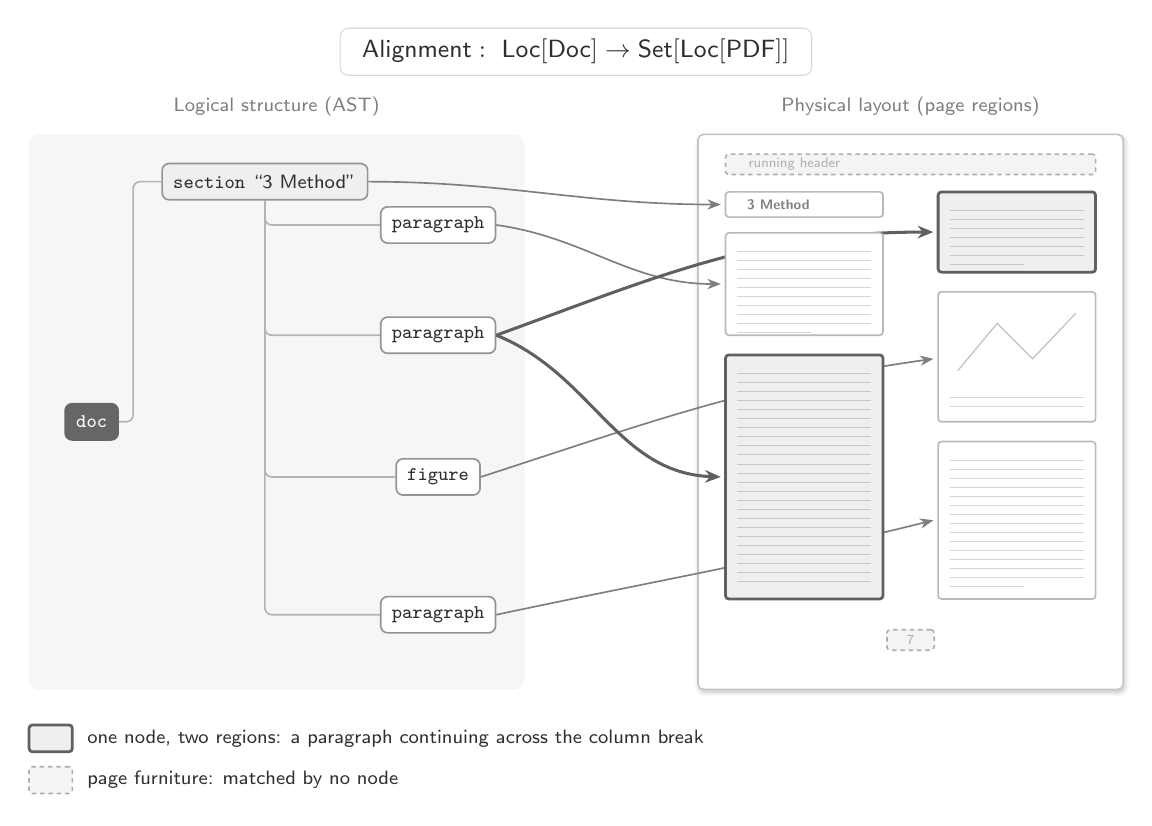
\begin{tikzpicture}

% ============================ title badge ==================================
\node[rounded corners=3pt, draw=inkSoft!30, fill=white, inner xsep=8pt,
      inner ysep=4pt, font=\small] at (6.95,8.00)
     {$\mathsf{Alignment}:\ \mathsf{Loc}[\mathsf{Doc}] \rightarrow
       \mathsf{Set}[\mathsf{Loc}[\mathsf{PDF}]]$};

\node[grouplbl] at (3.15,7.30) {Logical structure (AST)};
\node[grouplbl] at (11.20,7.30) {Physical layout (page regions)};

% ============================ the two cards ================================
\fill[softcard, fill=astFill!55] (0.00,-0.10) rectangle (6.30,6.95);
\node[page, fit={(8.50,-0.10) (13.90,6.95)}, inner sep=0pt,
      blur shadow={shadow blur steps=8, shadow xshift=0.5pt,
                   shadow yshift=-0.9pt, shadow opacity=25}] {};

% ======================= LEFT: logical structure (AST) =====================
\node[astroot] (doc)  at (0.80,3.30) {\texttt{doc}};
\node[astsec]  (sec1) at (3.00,6.35) {\texttt{section} ``3 Method''};
\node[astnode] (p1)   at (5.20,5.80) {\texttt{paragraph}};
\node[astnode] (p2)   at (5.20,4.40) {\texttt{paragraph}};
\node[astnode] (fg)   at (5.20,2.60) {\texttt{figure}};
\node[astnode] (p3)   at (5.20,0.85) {\texttt{paragraph}};

\draw[asttree] (doc.east) -- ++(0.18,0) |- (sec1.west);
\foreach \c in {p1,p2,fg,p3}{ \draw[asttree] (sec1.south) |- (\c.west); }

% ============================= THE MAPPING =================================
% (drawn before the regions, so the links pass behind them)
\draw[maplink] (sec1.east) to[out=0,in=180]   (8.79,6.06);
\draw[maplink] (p1.east)   to[out=-8,in=180]  (8.79,5.05);
\draw[maplink] (fg.east)   to[out=18,in=188]  (11.49,4.10);
\draw[maplink] (p3.east)   to[out=12,in=194]  (11.49,2.05);

% one node, two regions, split across the column break
\draw[maphot]  (p2.east) to[out=-22,in=178] (8.79,2.60);
\draw[maphot]  (p2.east) to[out=20,in=180]  (11.49,5.71);

% ======================= page regions (opaque, on top) =====================
\node[furniture, fit={(8.85,6.44) (13.55,6.70)}, inner sep=0pt] {};
\node[font=\tiny, text=mutedLine, anchor=west] at (9.02,6.57) {running header};
\node[furniture, fit={(10.90,0.40) (11.50,0.66)}, inner sep=0pt] {};
\node[font=\tiny, text=mutedLine] at (11.20,0.53) {7};

% --- left column ---
\node[lbox, fit={(8.85,5.90) (10.85,6.22)}, inner sep=0pt] {};
\node[font=\tiny, text=pdfLine, anchor=west] at (9.00,6.06) {\textbf{3 Method}};

\node[lbox, fit={(8.85,4.40) (10.85,5.70)}, inner sep=0pt] {};
\fakepara{9.00}{5.58}{1.70}{9}

\node[lboxhi, fit={(8.85,1.05) (10.85,4.15)}, inner sep=0pt] {};
\fakelines[hotLine!35]{9.00}{4.03}{1.70}{24}

% --- right column ---
\node[lboxhi, fit={(11.55,5.20) (13.55,6.22)}, inner sep=0pt] {};
\fakepara[hotLine!35]{11.70}{6.10}{1.70}{6}

\node[lbox, fit={(11.55,3.30) (13.55,4.95)}, inner sep=0pt] {};
\draw[pdfLine!45, line width=0.5pt, line join=round]
      (11.80,3.95) -- (12.30,4.55) -- (12.75,4.10) -- (13.30,4.68);
\fakelines{11.70}{3.72}{1.70}{2}

\node[lbox, fit={(11.55,1.05) (13.55,3.05)}, inner sep=0pt] {};
\fakepara{11.70}{2.93}{1.70}{14}

% ================================ legend ===================================
\node[lboxhi, minimum width=5.5mm, minimum height=3.4mm, inner sep=0pt]
      at (0.28,-0.72) {};
\node[caption, anchor=west] at (0.62,-0.72)
     {one node, two regions: a paragraph continuing across the column break};

\node[furniture, minimum width=5.5mm, minimum height=3.4mm, inner sep=0pt]
      at (0.28,-1.25) {};
\node[caption, anchor=west] at (0.62,-1.25)
     {page furniture: matched by no node};

\end{tikzpicture}
\end{document}
"
\ifdefined\GRAYFIGS
  \usepackage[gray]{xcolor}
\else
  \usepackage{xcolor}
\fi
\usetikzlibrary{arrows.meta,positioning,fit,backgrounds,calc,shapes.geometric,
                shapes.misc,decorations.pathreplacing,patterns,matrix,shadows.blur}

% ------------------------------- palette -----------------------------------
\definecolor{ink}{HTML}{22333F}        % primary text
\definecolor{inkSoft}{HTML}{6B8299}    % secondary text, hairlines
\definecolor{astLine}{HTML}{2C7A9B}    % logical view
\definecolor{astFill}{HTML}{E7F2F7}
\definecolor{pdfLine}{HTML}{B0762F}    % physical view
\definecolor{pdfFill}{HTML}{FBF2E3}
\definecolor{hotLine}{HTML}{B03A55}    % the emphasised relation
\definecolor{hotFill}{HTML}{FBE9EC}
\definecolor{mutedLine}{HTML}{9FB3C8}  % furniture / unmatched
\definecolor{mutedFill}{HTML}{F1F5F8}

\tikzset{
  every node/.append style = {text=ink},
  >=Stealth,
  % --- logical structure (AST) -------------------------------------------
  astnode/.style   = {draw=astLine!70, fill=white, rounded corners=2.5pt,
                      line width=0.6pt, font=\scriptsize,
                      inner xsep=4pt, inner ysep=2.5pt, minimum height=4.6mm},
  astroot/.style   = {astnode, fill=astLine, draw=astLine, text=white},
  astsec/.style    = {astnode, fill=astFill},
  asttree/.style   = {draw=astLine!50, line width=0.6pt, rounded corners=2.5pt},
  % --- physical layout (page regions) ------------------------------------
  page/.style      = {draw=inkSoft!45, fill=white, line width=0.6pt,
                      rounded corners=2pt},
  lbox/.style      = {draw=pdfLine!55, fill=white, line width=0.6pt,
                      rounded corners=1.2pt},
  lboxhi/.style    = {draw=hotLine, fill=hotFill, line width=1.0pt,
                      rounded corners=1.2pt},
  furniture/.style = {draw=mutedLine, dash pattern=on 1.6pt off 1.4pt,
                      fill=mutedFill, line width=0.6pt, rounded corners=1.2pt},
  % --- relations ----------------------------------------------------------
  maplink/.style   = {draw=inkSoft, line width=0.6pt,
                      -{Stealth[length=1.7mm,width=1.3mm]}},
  maphot/.style    = {draw=hotLine, line width=1.1pt,
                      -{Stealth[length=2mm,width=1.6mm]}},
  flow/.style      = {draw=inkSoft, line width=0.7pt,
                      -{Stealth[length=2mm,width=1.6mm]}, rounded corners=2pt},
  % --- pipeline stages ----------------------------------------------------
  stage/.style     = {draw=inkSoft!55, fill=white, rounded corners=2.5pt,
                      font=\scriptsize, align=center, inner sep=3.5pt,
                      minimum height=7mm, text width=32mm},
  artefact/.style  = {draw=inkSoft!35, fill=mutedFill, rounded corners=2.5pt,
                      font=\scriptsize, align=center, inner sep=3.5pt,
                      minimum height=7mm, text width=32mm},
  % --- labels -------------------------------------------------------------
  grouplbl/.style  = {font=\scriptsize, text=inkSoft},
  caption/.style   = {font=\scriptsize, text=ink},
  tinylbl/.style   = {font=\tiny, text=inkSoft},
  softcard/.style  = {rounded corners=4pt, draw=none},
}

% Fake text lines inside a layout box.
% [colour] {x} {y top} {width} {line count}
\newcommand{\fakelines}[5][pdfLine!32]{%
  \foreach \fli in {1,...,#5}{%
    \draw[#1, line width=0.32pt] (#2,{#3-0.115*\fli}) -- ++({#4},0);}%
}
% Same, with a short final line (end of a paragraph)
\newcommand{\fakepara}[5][pdfLine!32]{%
  \foreach \fli in {1,...,#5}{%
    \draw[#1, line width=0.32pt] (#2,{#3-0.115*\fli}) -- ++({#4},0);}%
  \draw[#1, line width=0.32pt] (#2,{#3-0.115*(#5+1)}) -- ++({0.55*#4},0);%
}

\begin{document}
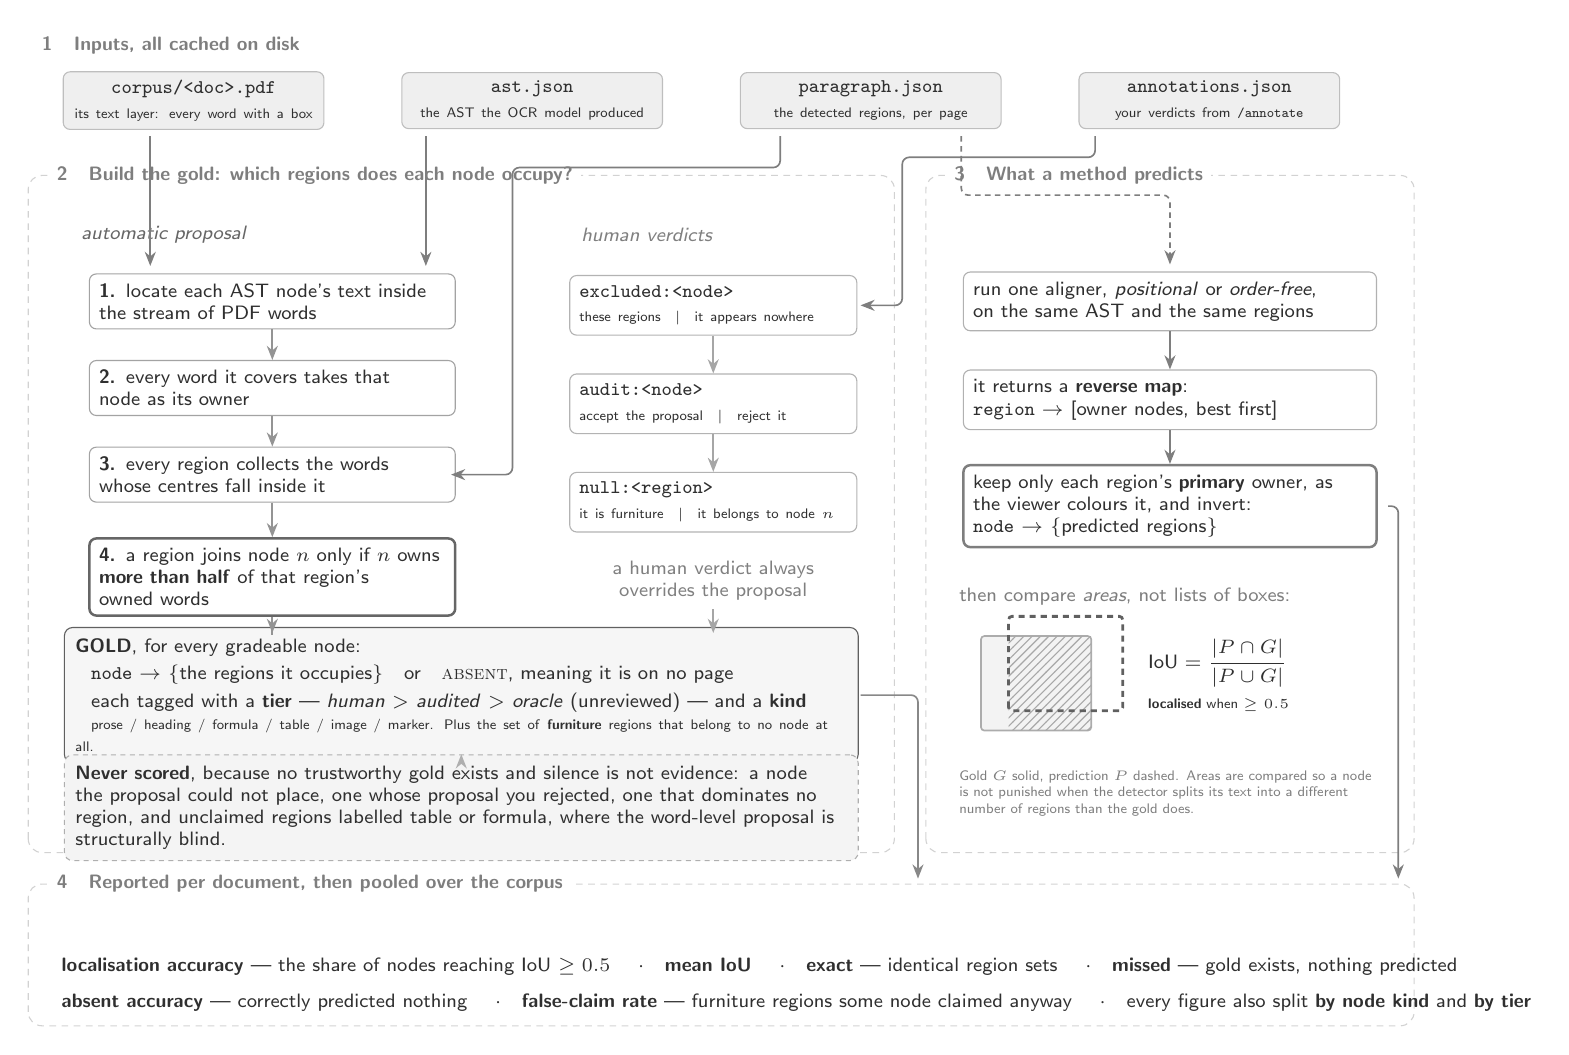
\begin{tikzpicture}[
  inp/.style   = {draw=inkSoft!50, fill=inkSoft!12, rounded corners=2.5pt,
                  align=center, font=\scriptsize, inner sep=3pt, text width=31mm},
  ostep/.style = {draw=astLine!60, fill=white, rounded corners=2.5pt,
                  align=left, font=\scriptsize, inner sep=3.5pt, text width=44mm},
  hstep/.style = {draw=pdfLine!60, fill=white, rounded corners=2.5pt,
                  align=left, font=\scriptsize, inner sep=3.5pt, text width=34mm},
  pstep/.style = {draw=inkSoft!60, fill=white, rounded corners=2.5pt,
                  align=left, font=\scriptsize, inner sep=3.5pt, text width=50mm},
  goldbox/.style = {draw=hotLine, fill=hotFill!55, rounded corners=3pt,
                  align=left, font=\scriptsize, inner sep=4pt, text width=98mm},
  dropbox/.style = {draw=mutedLine, dash pattern=on 1.8pt off 1.6pt,
                  fill=mutedFill, rounded corners=3pt, align=left,
                  font=\scriptsize, inner sep=4pt, text width=98mm},
  zone/.style  = {rounded corners=5pt, draw=inkSoft!35,
                  dash pattern=on 2.4pt off 2pt},
  ztitle/.style= {font=\scriptsize\bfseries, text=inkSoft, fill=white,
                  inner xsep=3pt, inner ysep=1pt},
  ar/.style    = {draw=inkSoft, line width=0.6pt,
                  -{Stealth[length=1.8mm,width=1.4mm]}, rounded corners=2.5pt},
]

% ================================ zones ====================================
\draw[zone] (0.05,2.35) rectangle (11.05,10.95);
\draw[zone] (11.45,2.35) rectangle (17.65,10.95);
\draw[zone] (0.05,0.15) rectangle (17.65,1.95);

% ============================== 1. INPUTS ==================================
\node[font=\scriptsize\bfseries, text=inkSoft, anchor=west] at (0.10,12.60)
     {1\quad Inputs, all cached on disk};
\node[inp] (inPdf) at (2.15,11.90)
     {\texttt{corpus/<doc>.pdf}\\[1pt]\tiny its text layer: every word with a box};
\node[inp] (inAst) at (6.45,11.90)
     {\texttt{ast.json}\\[1pt]\tiny the AST the OCR model produced};
\node[inp] (inReg) at (10.75,11.90)
     {\texttt{paragraph.json}\\[1pt]\tiny the detected regions, per page};
\node[inp] (inAnn) at (15.05,11.90)
     {\texttt{annotations.json}\\[1pt]\tiny your verdicts from \texttt{/annotate}};

% ======================= 2. GOLD CONSTRUCTION ==============================
\node[ztitle, anchor=west] at (0.30,10.95)
     {2\quad Build the gold: which regions does each node occupy?};

\node[font=\scriptsize\itshape, text=astLine, anchor=west] at (0.60,10.20)
     {automatic proposal};
\node[ostep] (o1) at (3.15,9.35)
     {\textbf{1.} locate each AST node's text inside\\ the stream of PDF words};
\node[ostep] (o2) at (3.15,8.25)
     {\textbf{2.} every word it covers takes that\\ node as its owner};
\node[ostep] (o3) at (3.15,7.15)
     {\textbf{3.} every region collects the words\\ whose centres fall inside it};
\node[ostep, draw=astLine, line width=0.9pt] (o4) at (3.15,5.85)
     {\textbf{4.} a region joins node $n$ only if $n$ owns\\
      \textbf{more than half} of that region's\\ owned words};
\foreach \a/\b in {o1/o2, o2/o3, o3/o4}{\draw[ar, draw=astLine!70] (\a) -- (\b);}

\node[font=\scriptsize\itshape, text=pdfLine, anchor=west] at (6.95,10.20)
     {human verdicts};
\node[hstep] (h1) at (8.75,9.30)
     {\texttt{excluded:<node>}\\[1pt]\tiny these regions \ $|$ \ it appears nowhere};
\node[hstep] (h2) at (8.75,8.05)
     {\texttt{audit:<node>}\\[1pt]\tiny accept the proposal \ $|$ \ reject it};
\node[hstep] (h3) at (8.75,6.80)
     {\texttt{null:<region>}\\[1pt]\tiny it is furniture \ $|$ \ it belongs to node $n$};
\node[font=\scriptsize, text=pdfLine, align=center] at (8.75,5.80)
     {a human verdict always\\ overrides the proposal};
\draw[ar, draw=pdfLine!70] (h1) -- (h2);
\draw[ar, draw=pdfLine!70] (h2) -- (h3);

\node[goldbox] (gold) at (5.55,4.35)
     {\textbf{GOLD}, for every gradeable node:\\[2pt]
      \hspace*{2mm}\texttt{node} $\rightarrow$ \{the regions it occupies\}\quad or\quad
      \textsc{absent}, meaning it is on no page\\[2pt]
      \hspace*{2mm}each tagged with a \textbf{tier} --- \emph{human} $>$ \emph{audited} $>$
      \emph{oracle} (unreviewed) --- and a \textbf{kind}\\
      \hspace*{2mm}\tiny prose / heading / formula / table / image / marker.
      Plus the set of \textbf{furniture} regions that belong to no node at all.};
\draw[ar, draw=astLine!70] (o4.south) -- ++(0,-0.28) -| (3.15,5.14);
\draw[ar, draw=pdfLine!70] (8.75,5.44) -- (8.75,5.14);

\node[dropbox] (drop) at (5.55,2.92)
     {\textbf{Never scored}, because no trustworthy gold exists and silence is
      not evidence: a node the proposal could not place, one whose proposal you
      rejected, one that dominates no region, and unclaimed regions labelled
      table or formula, where the word-level proposal is structurally blind.};
\draw[ar, draw=mutedLine] (gold) -- (drop);

% ========================== 3. WHAT A METHOD PREDICTS ======================
\node[ztitle, anchor=west] at (11.70,10.95) {3\quad What a method predicts};

\node[pstep] (p1) at (14.55,9.35)
     {run one aligner, \emph{positional} or \emph{order-free},\\
      on the same AST and the same regions};
\node[pstep] (p2) at (14.55,8.10)
     {it returns a \textbf{reverse map}:\\
      \texttt{region} $\rightarrow$ [owner nodes, best first]};
\node[pstep, draw=inkSoft, line width=0.9pt] (p3) at (14.55,6.75)
     {keep only each region's \textbf{primary} owner, as\\
      the viewer colours it, and invert:\\
      \texttt{node} $\rightarrow$ \{predicted regions\}};
\draw[ar] (p1) -- (p2);
\draw[ar] (p2) -- (p3);

\node[font=\scriptsize, text=inkSoft, anchor=west] at (11.75,5.60)
     {then compare \emph{areas}, not lists of boxes:};
\draw[draw=pdfLine!65, fill=pdfFill, line width=0.6pt, rounded corners=1.2pt]
     (12.15,3.90) rectangle (13.55,5.10);
\begin{scope}
  \clip (12.15,3.90) rectangle (13.55,5.10);
  \fill[pattern=north east lines, pattern color=hotLine!55]
       (12.50,3.90) rectangle (13.55,5.10);
\end{scope}
\draw[dash pattern=on 2.2pt off 1.8pt, draw=hotLine, line width=1.0pt,
      rounded corners=1.2pt] (12.50,4.15) rectangle (13.95,5.35);
\node[font=\scriptsize, anchor=west, align=left] at (14.15,4.60)
     {$\mathsf{IoU}=\dfrac{|P\cap G|}{|P\cup G|}$\\[3pt]
      \tiny \textbf{localised} when $\geq 0.5$};
\node[font=\tiny, text=inkSoft, anchor=west, align=left, text width=53mm]
     at (11.75,3.10)
     {Gold $G$ solid, prediction $P$ dashed. Areas are compared so a node is not
      punished when the detector splits its text into a different number of
      regions than the gold does.};

% ============================== 4. METRICS =================================
\node[ztitle, anchor=west] at (0.30,1.95)
     {4\quad Reported per document, then pooled over the corpus};
\node[font=\scriptsize, anchor=west, align=left] at (0.35,0.90)
     {\textbf{localisation accuracy} --- the share of nodes reaching IoU
      $\geq 0.5$ \quad$\cdot$\quad \textbf{mean IoU} \quad$\cdot$\quad
      \textbf{exact} --- identical region sets \quad$\cdot$\quad
      \textbf{missed} --- gold exists, nothing predicted};
\node[font=\scriptsize, anchor=west, align=left] at (0.35,0.45)
     {\textbf{absent accuracy} --- correctly predicted nothing \quad$\cdot$\quad
      \textbf{false-claim rate} --- furniture regions some node claimed anyway
      \quad$\cdot$\quad every figure also split \textbf{by node kind} and
      \textbf{by tier}};

% ----------------------------- input wiring --------------------------------
\draw[ar] (1.60,11.45) -- (1.60,9.80);
\draw[ar] (5.10,11.45) -- (5.10,9.80);
\draw[ar] (9.60,11.45) -- (9.60,11.05) -- (6.20,11.05) -- (6.20,7.15) -- (5.42,7.15);
\draw[ar] (13.60,11.45) -- (13.60,11.18) -- (11.15,11.18) -- (11.15,9.30) -- (10.62,9.30);
\draw[ar, dash pattern=on 2pt off 1.6pt]
     (11.90,11.45) -- (11.90,10.70) -- (14.55,10.70) -- (14.55,9.82);

% gold and prediction meet in the metrics band
\draw[ar, draw=hotLine!75] (10.62,4.35) -- (11.35,4.35) -- (11.35,2.02);
\draw[ar] (17.32,6.75) -- (17.45,6.75) -- (17.45,2.02);

\end{tikzpicture}
\end{document}
